DOM

\section{Wizualizacja}
\label{sec:wizualizacja}

Poniższa sekcja zawiera próbę analizy dostępnych metod prezentacji danych zarówno zbiorów punktów, zdjęć i animacji. Główną uwagę zwrócono na 3 główne sposoby wizualizacji grafik. Ostatnia część zawiera zbiór dostępnych funkcjonalności, stanowi przewodnik po dostępnych możliwościach i ukazuje w jaki sposób można personalizować dane.


\subsection{Rodzaje map}
\label{subsec:Rodzaje map}

Tworząc aplikację która ma dostarczać informacji korzystających z map należy zapoznać się dostępnymi źródłami. Z powodu szrokiego wyboru poniżej omówione zostaną jedynie aplikacje które dostarczają informacji ogólnoświatowych. Na polskim rynku dostępnych jest kilka rozwiązań, ich główną wadą jest ograniczenie do terytorium Polski, dodatkowo często nie dostarczają one obrazów satelitarnych, są to m.in. \underline{\texttt{http://zumi.pl}}
\ref{}

\subsubsection{Google Maps}
\label{subsubsec:Google Maps}
\nocite{googlemapsbegin}
Rysunek \ref{fig:googleMaps_1} przedstawia obraz otrzymany w aplikacji Google Maps. Dodatkowo włączona opcja prezentacji natężenia ruchu jedynie potwierdza duże możliwości i łatwość obsługi. Przyjazny interfejs sprawia że praca jest prosta i pozwala na osiągnięcie bardzo dobrych wyników.


\begin{figure}[H]
  \centering
    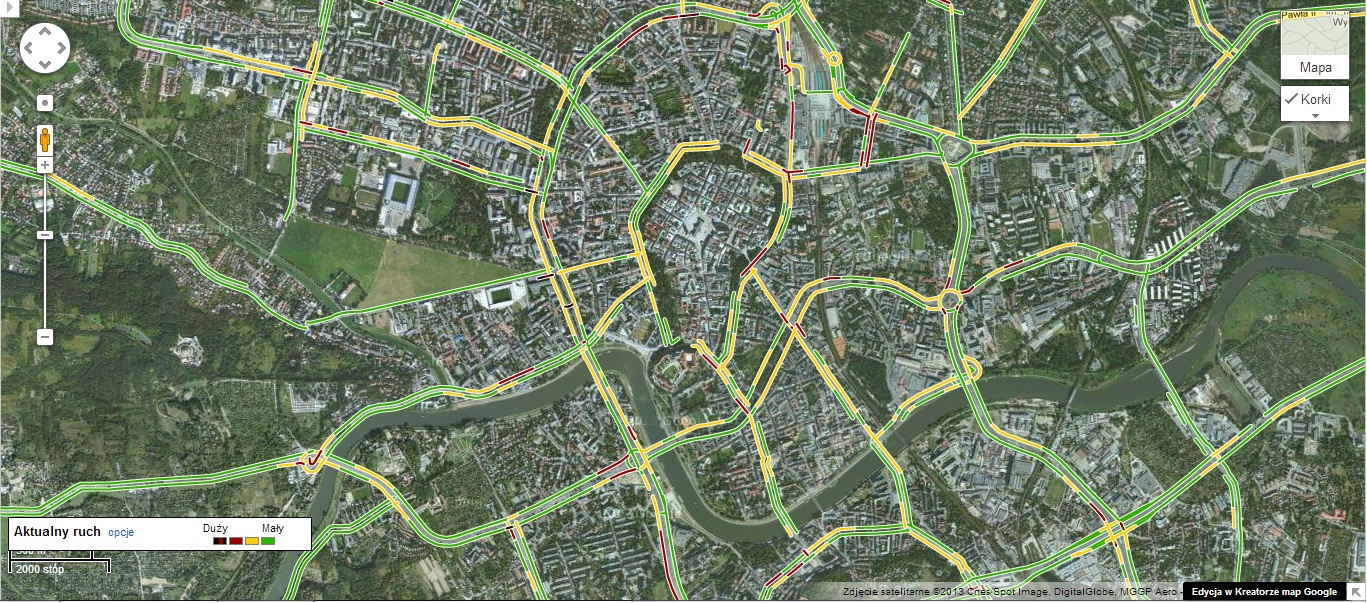
\includegraphics[width=100mm]{ge/gm_1.jpg}
  \caption{Google Maps.}
  \label{fig:googleMaps_1}
\end{figure}


\subsubsection{Windows Maps}
\label{subsubsec:Windows Maps}

Rysunek \ref{fig:bingMaps_1} przedstawia obraz otrzymany wykorzystując Bing Maps. W tym konkretnym przykładzie widzimy znaczną różnicę kolorów, obecność chmur pomniejsza wartość tych zdjęć. Należy wspomnieć o znacznie uboższym interfejsie dostarczanym użytkownikowi, interakcja jest w znacznym stopniu uboższa.

\begin{figure}[H]
  \centering
    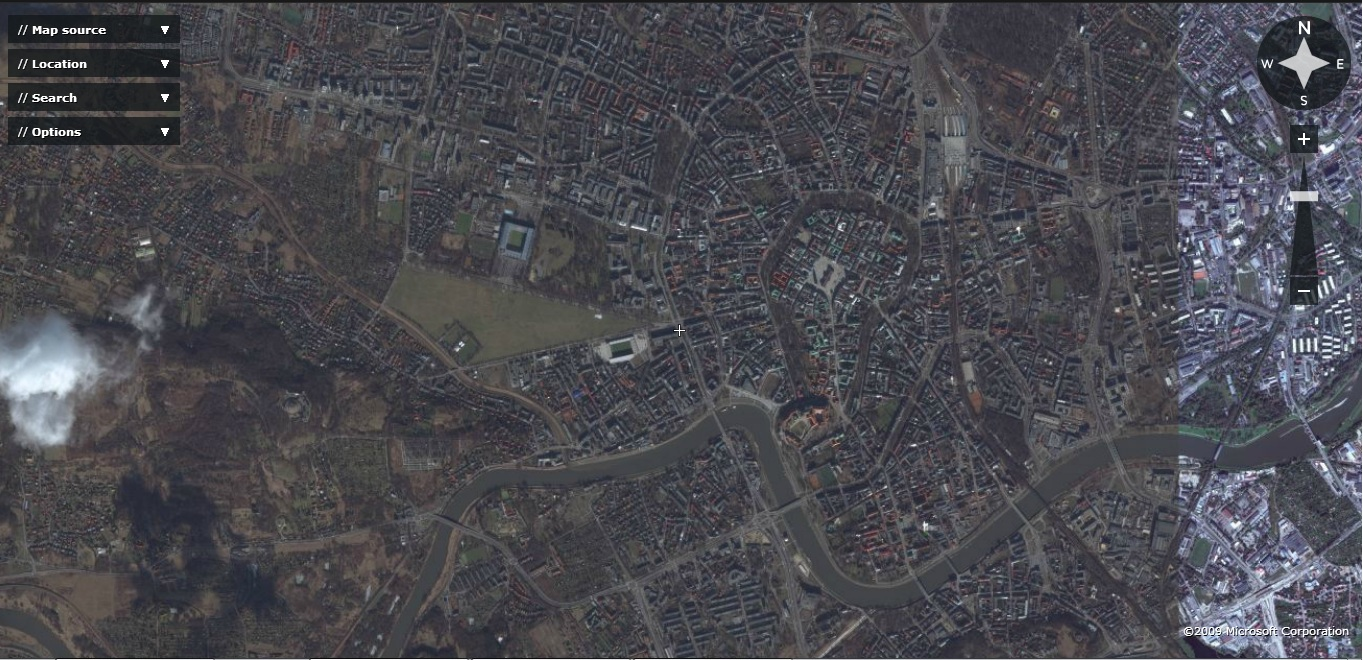
\includegraphics[width=100mm]{ge/bing_1.jpg}
  \caption{Bing Maps.}
  \label{fig:bingMaps_1}
\end{figure}

\subsubsection{Yahoo Maps}
\label{subsubsec:Yahoo Maps}

Kolejnym dostarczycielem danych kartograficznym jest Yahoo, przykład znajduje się na rysunku \ref{fig:yahooMaps_1}. Interfejs jest zbliżony do Bing Maps, jednak obszar na którym możemy przedlądać zdjęcia jest mniejszy, obszary oddalone od większych miast nie są w pełni uwzglęnione. Z tego powodu nie stanowi w pełni akceptowalnej alterantywy.

\begin{figure}[H]
  \centering
    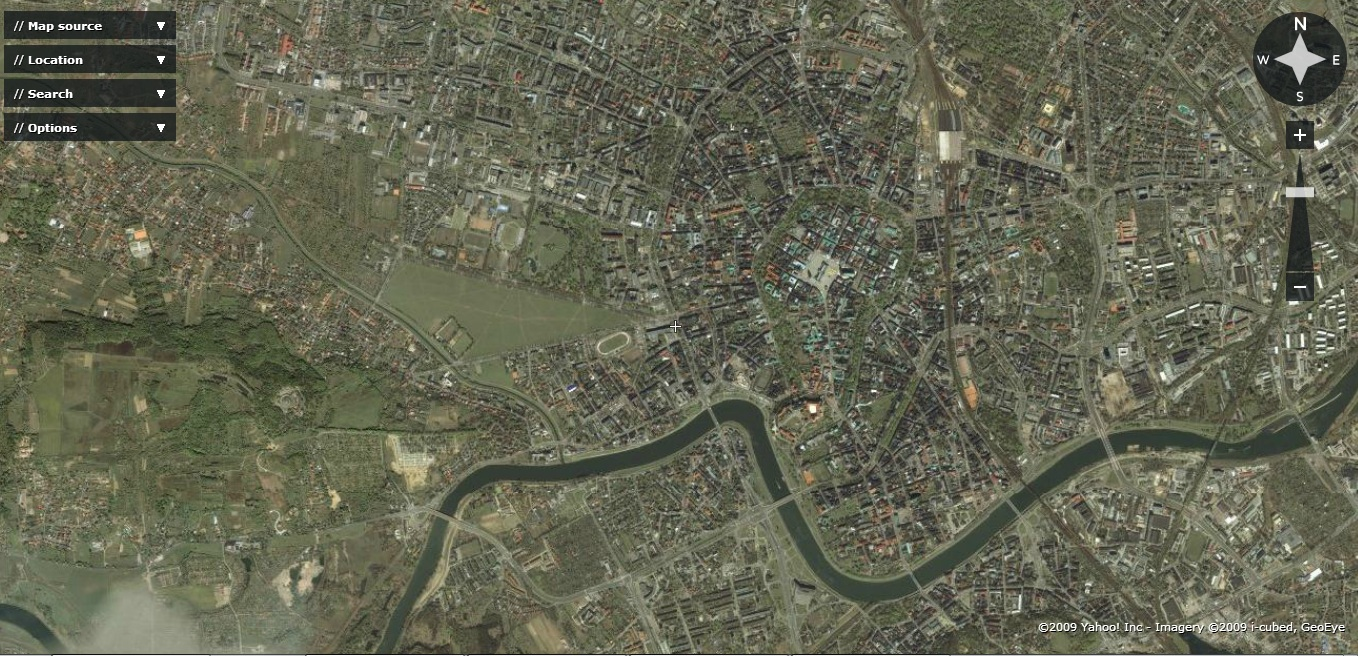
\includegraphics[width=100mm]{ge/yahoo_1.jpg}
  \caption{Yahoo Maps.}
  \label{fig:yahooMaps_1}
\end{figure}


\subsubsection{Apple Maps}
\label{subsubsec:Apple Maps}

Kolejną dużą marką która dostarcza informację jest Apple. Niestety nie ma wersji która pozwalałaby na dostęp do tej usługi z powszechnie używanych komputerów stacjonarnych. Dodatkowo jakość dostarczanych informacji jest bardzo złej jakości.


\subsection{Metody prezentacji}
\label{subsec:presentation}

Poniższa sekcja zawiera opis dostępnych metod służących do prezentacji danych w przeglądarce internetowej. Przedstawia zalety jak i wady każdego z rozwiązań.


\subsubsection{Flash}
\label{subsubsec:graphicFlash}


Wadą tego rozwiązania wynikająca ze specyfikacji całego języka jest bardzo słaba integracja z dokumentami HTML, nie możliwa jest pełna iterakcja z pozostałymi elementani na stronie. Problem ten nie dotyczy kolejnego podejścia \ref{subsec:svg}

\subsubsection{Canvas}
\label{subsubsec:canvas}


Bardzo ciekawym i wartym zainteresowania dodanym elementem w nowej wersji HTML jest obecność znaczniku canvas. Pozwala on na dynamiczne , skryptowe renderowanie kształtów i obrazów. Dzięki temu obiektowi możliwe stało się tworzenie animacji czy nawet gier działających w przeglądarce bez konieczności używania dodatkowych wtyczek czy programów.

\underline{\texttt{http://techtrendy.pl/title, Pierwsza-gra-3D-napisana-w-HTML5,wid,14102779,wiadomosc.html?ticaid=6107dc}}

Przykładem wielkich możliwości jakie dostarcza udoskonalony język jest fakt iż już w roku 2011 powstała pierwsza trójwymiarowa gra stworzona w całości przy użyciu HTML5. Przykład grafiki widoczny jest na rysunku \ref{fig:html3d}.

\begin{figure}[H]
  \centering
    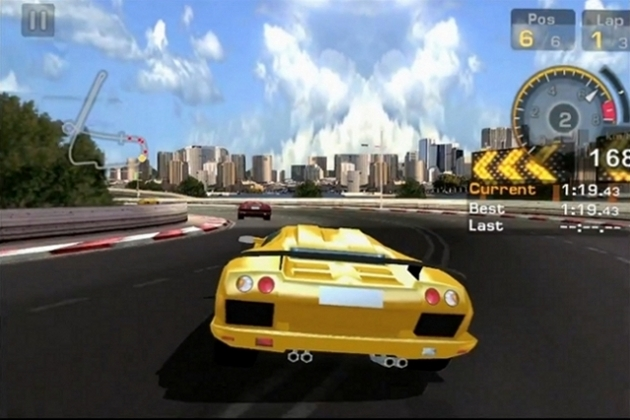
\includegraphics[width=100mm]{ge/html5_3d.jpg}
  \caption{Pierwsza gra 3D w html5.}
  \label{fig:html3d}
\end{figure}

Funkcjonalnością która wydaje się być szczególnie przydatna w stosunku do omawianego projektu jest możliwość rysowania kształtów geomeycznych. Przykładem wykorzystania tej technologi jest \ref{fig:canvas1} na którym przy pomocy okręgu zaznaczono rynek główny w Krakowie i jego okolice, możliwość zmiany transparentości narysowanego kształtu pozwala aby obraz podnim był nadal widoczny.

Niestety rozwiązanie to nie może zostać wykorzystane wraz z wybranym modelem prezentacji danych geograficznych. Rysunek \ref{fig:canvas1} prezentuje potencjlne możliwośći jednak nawet analiza listeningu \ref{lst:canvas} wskazuje podstawowe wymaganie wykorzystanie tego rozwiązania. Bazowy element w obrębie którego możliwa jest akcja musi być elementem canvas.
Otrzymany efekt jest wynikiem wykorzystania statycznego obrazu który został zaimportowany z pamięci komputera i wykorzystany jako tło. Zabieg ten pozwala nazaprezentowanie możliwości rozwiąznia ale uniemżliwia wykorzystanie funkcjonalności które dostarczane są przez Google Maps(zmiana punktu patrzenia, stopnia przybliżenia i inne). Z tego powodu zdecydowano się na zaprzestanie prac z tym konketnym rozwiązaniem i nie wykorzystanie go w docelowej aplikacji.

  \begin{figure}[H]
  \centering
    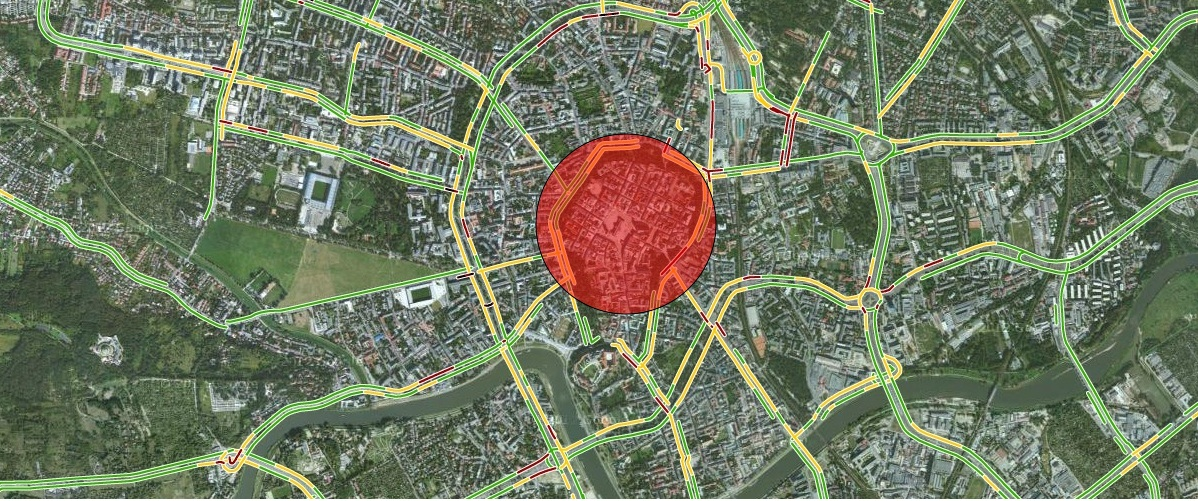
\includegraphics[width=100mm]{ge/canvas1.jpg}
  \caption{Zaznaczenie przez canvas}
  \label{fig:canvas1}
\end{figure}

\lstset{language=JavaScript}
\begin{lstlisting}[label={lst:canvas},caption={json}]

      var canvas = document.getElementById('myCanvas');
      var context = canvas.getContext('2d');
      var imageObj = new Image();
	
      imageObj.onload = function() {
      context.drawImage(imageObj, 69, 50);
	  context.beginPath();
      context.arc(canvas.width / 2, canvas.height / 2, 90, 0, 2 * Math.PI, false);
      context.fillStyle = "rgba(255, 0, 0, 0.5)";
      context.fill();
      context.stroke();
      };
      imageObj.src = './gm_1.jpg';
      .
      .
      .
      <canvas id="myCanvas" width="200" height="100">
      </canvas>
\end{lstlisting}

\subsubsection{SVG}
\label{subsubsec:svg}

SVG(en. Scalable Vector Graphics) do prezentacji danych, tworzenia animacji i płynnych zmian kształtów. Jest to powszechnie dostępny format zapisu grafiki wektorowej który oprócz prostych kształtów geometrycznych pozwala na korzystanie z zaawansowanych filtrów i efektów.

Wykorzystywany jest wektorowy format zapisu danych, został on dokładniej omówiony w sekcji \ref{subsec:zapisWektorowy}.
W wyniku takiego zabiegu plik svg opisujący obraz graficzny ma znacznie mniejszy rozmiar od oryginalnego, jednocześnie niezależnie od wielkości jego jakość jest taka sama.

Autorzy artykułu "Zastosowanie języka SVG do wizualizacji danych geoprzestrzennych" \cite{svgUse} zwracają również uwagę na tekstwoy format zapisu, jest on mniej oszczędny niż binarny ale pozwala na edycję dowolnym edytorem tekstu co pozwala na przeszukiwanie zawartości np. wyszikiwarkom internetowym.

W celach porównawczych wykorzystano logo AGH \ref{fig:aghlogo} o rozmiarach 305x591 pikseli o gęstości 150 dpi (en. Dots per inch, określa ilość indywidualnych punktów na odcinu jednego cala, 2.54cm), po zapisie na dysku twardym zajmował on 75 KB pamięci. Następnie wykoano zapis grafiki w testowanym formacie zajmował on 3KB , efekt został przedstawiony w listingu \ref{lst:logoaghsvg}.



\begin{figure}[H]
  \centering
    
\includegraphics[width=30mm]{ge/agh_logo.jpg}
  \caption{Logo AGH}
  \label{fig:aghlogo}
\end{figure}

\lstset{language=JavaScript}
\begin{lstlisting}[label={lst:logoaghsvg},caption={Logo AGH w zapisie SVG.}]

<svg xmlns="http://www.w3.org/2000/svg" version="1.1">
<g transform="translate(0.000000,591.000000) scale(0.100000,-0.100000)" fill="#1e1e1e" stroke="none">
<path d="M984 5863 c70 -97 112 -224 143 -429 15 -97 17 -289 20 -1761 l4 -1653 99 0 100 0 0 1543 c0 933 -4 1594 -10 1673 -12 158 -37 262 -89 369 -61 127 -136 208 -265 285 l-38 23 36 -50z"/>
<path d="M1115 5878 c164 -131 256 -283 306 -503 l23 -100 3 -1627 4 -1628 94 0 95 0 0 1618 c-1 1317 -3 1631 -14 1692 -50 274 -208 455 -485 556 l-66 24 40 -32z"/>
<path  d="M1317 5867 c208 -110 326 -253 395 -477 l23 -75 3 -1647 2 -1648 100 0 100 0 0 1609 c0 1744 2 1676 -54 1826 -62 163 -173 282 -343 368 -57 29 -193 71 -263 81 -44 6 -44 5 37 -37z"/>
<path fill="#00693c" d="M52 3578 l3 -1433 23 -79 c76 -271 252 -444 522 -515 146 -38 153 -36 65 15 -170 97 -261 190 -331 339 -84 180 -78 49 -81 1668 l-3 1437 -100 0 -101 0 3 -1432z"/>
<path fill="#00693c" d="M350 3622 c0 -909 4 -1417 11 -1472 12 -101 54 -228 100 -307 73 -124 220 -238 384 -298 l70 -26 -35 27 c-61 47 -164 160 -199 218 -61 102 -100 219 -121 361 -6 44 -10 594 -10 1478 l0 1407 -100 0 -100 0 0 -1388z"/>
<path fill="#00693c" d="M650 3607 c0 -906 4 -1433 10 -1487 35 -282 148 -465 368 -594 8 -5 -3 14 -22 42 -74 103 -115 233 -141 452 -13 106 -15 346 -15 1558 l0 1432 -100 0 -100 0 0 -1403z"/>
<path fill="#a71930" d="M2237 3518 c-3 -1478 -3 -1494 -25 -1604 -27 -139 -69 -258 -121 -334 l-39 -60 40 23 c68 37 186 155 228 226 21 36 50 101 65 143 55 168 55 152 55 1686 l0 1412 -100 0 -99 0 -4 -1492z"/>
<path fill="#a71930" d="M2537 3563 c-3 -1354 -4 -1453 -21 -1523 -50 -211 -144 -362 -301 -488 l-40 -32 65 24 c255 93 402 249 472 501 l23 80 3 1443 3 1442 -101 0 -100 0 -3 -1447z"/>
<path fill="#a71930" d="M2838 3573 l-3 -1438 -23 -80 c-63 -228 -190 -384 -403 -498 -83 -44 -75 -45 56 -12 292 74 468 241 547 521 l23 79 3 1433 3 1432 -100 0 -100 0 -3 -1437z"/>
<path d="M1480 925 c-307 -69 -464 -387 -331 -670 101 -216 388 -308 704 -224 l38 10 -3 225 -3 226 -33 29 c-32 28 -35 29 -142 29 l-111 0 23 -31 c21 -29 23 -42 26 -199 l3 -169 -25 -7 c-58 -14 -155 23 -199 75 -48 58 -70 135 -71 251 -1 96 1 110 27 162 31 64 71 102 136 131 60 26 195 21 260 -11 25 -12 46 -22 48 -22 2 0 3 40 3 88 l0 89 -37 12 c-60 20 -238 23 -313 6z"/>
<path d="M244 889 c14 -17 26 -39 26 -49 0 -10 -61 -197 -135 -416 -74 -219 -135 -400 -135 -401 0 -2 38 -3 85 -3 l84 0 34 108 35 107 150 3 150 3 37 -111 37 -110 128 0 129 0 -29 83 c-97 284 -244 690 -265 732 -37 77 -58 85 -220 85 l-137 0 26 -31z m201 -369 c24 -71 41 -131 37 -134 -8 -9 -192 -7 -192 1 0 4 21 71 47 150 34 103 50 138 56 127 5 -9 28 -74 52 -144z"/>
<path d="M2263 883 c22 -37 22 -45 25 -450 l3 -413 120 0 119 0 0 190 0 190 135 0 135 0 0 -190 0 -190 120 0 120 0 0 450 0 450 -120 0 -120 0 0 -185 0 -185 -134 0 -134 0 -4 148 c-3 158 -9 176 -59 206 -20 12 -53 16 -128 16 l-100 0 22 -37z"/>
</g>
</svg>

\end{lstlisting}

\subsubsection{Google Maps Overlay}
\label{subsubsec:overlays}

Wraz z wykorzystaniem Google Maps jako bazowym źródłem danych otrzymujemy API(en.Application programming interface) umożliwiające tworzenie różnego rodzaju elementów których wygląd można w dowolny sposób edytować i zmieniać według potrzeb użytkownika.W prosty sposób możliwe jest otrzymanie efektu który został stworzony przy pomocy canvas na rysunku \ref{fig:canvas1} zachowując pełną swobodę w dalszej pracy.

Pakiet google.maps zawiera kilka klas których zadaniem jest generowanie adekwatnych obiektów. Klasy te zostały omówione poniżej.

\begin{description}
\item[Marker] \hfill \\
    Pojedyńczy punkt na mapie o określonych właściwościach które można dowolnie edytować, tak aby jego wygląd, zachowanie i położenie było zgodne z oczekiwaniami.

\item[Polyline] \hfill \\
  Linia stworzona z dwóch lub więcej punktów. Tworzone odcinki mogą być liniami prostymi lub przedstawiać zakrzywienie ziemi, nie jest możliwe tworzenie bardziej skomplikowanych łuków.

\item[Polygon] \hfill \\
  Twrzy ciąg połączonych ze sobą punktów w określonej kolejności które tworzą zamknięty obszar. Określają obszar terenu który znajduje się wewnątrz figury.

\item[Circle] \hfill \\
  Na podstawie środka i jego promienia tworzy okrąg z obszarem wewnętrznym.

\item[Rectangle] \hfill \\
  Tworzy prostokąt posiadający przeciwległe boki w określonych punktach. Podobnie jak Polygon i Circle posiada obszar wewnętrzy którego właściwości graficzne można dowolnie definiować.

\item[OverlayView] \hfill \\
  Specjalna klasa służąca do wyświetlania własnych wartsw graficznych, takich jak zewnętrzny plik graficzny. Pozwala na łatwe łączenie ogólnodostępych danych jakimi są mapy z własnymi zdjęciami, rysunkami itp.

\end{description}

Intuicyjna i szybka edycja danych jest zapewniona poprzez udostępnianie klasy "DrawingManager". Tworzy ona dodatkowy element na ekranie użytkownika służący do pracy z wartwami znajdujacymi się na ekranie. Komponent ten wymaga jedynie wybrania odpowiedniego elementu a następnie wyznaczenie wymaganych informacji,zazwyczaj są to jeden lub dwa punkty niezbędne do stworzenia elementu. Pozostałe właściwości mogą być edytowane w dalszym etapie prac według wymagać.


\subsubsection{Oś czasu}
\label{subsubsec:os}

Tematem pracy oprócz wykorzystania i prezentacji danych na bazie informacji geograficznych jest ich połączenie z osią czasu, która pozwoliłaby na zmianę prezentowanych danych ze względu na interesujący nas okres czasu.

Ponieważ własna implementacja osi czasu która nieograniczałaby użytkownika, pozwala mu w pełni korzystać z możliwości pełnej aplikacji, która tylko w części składa się z możliwości manipulacji czasem postanowiono wykorzystać istniejące rozwiązanie.

Przeprowadzając badania rozwiązań głównymi aspektami na które zwrócono uwagę było:


\begin{itemize}

\item

Typ licencji
Niezwykle ważne jest aby końcowy projekt był całkowicie otwarty dla dalszego rozwoju, pozwalał użytkownikom na adaptację rozwiązań dla swoich potrzeb. Z uwagi na to licencja musi pozwalać na nieograniczoną modyfikację kodu źródłowego.

\item

Wykorzystywane technologie
Pamiętając że efektem końcowym powinien być framework odpowiadający szerokiemu gronowi odbiorców, będący jednocześnie darmowym ważne aby języki programowania wykorzystane przy jego tworzeniu też taki były. Oznacza to nie korzystanie z płatnych, wymagających licencji oprogramowań. Używane standarty powinny być rozpropagowane i używane przez szerokie grono obiorców.

\end{itemize}

Po długich i wnikliwych poszukiwaniach zdecydowano skorzystać z widget-u o nazwie Timeline który został stworzony przej projekt SIMILE działający na uczelni MIT. Pozwala on na bardzo dużą konfigurowalność dzięki czemu jego modyfikacja, nawet bez ingerencji w kod źródłowy jest bardzo prosta.
Projekt jest w stanie stworzyć kilka pasm któe będą określały interwały czasu. Pozwala to aby wynik końcowy był przejżysty bez względu czy prezentujemy wydarzenia które miały miejsce w okresie kilku minut czy setek lat.

Problemem który pojawił się było połączenie wybranego sposobu prezentacji osi czasu z mapą i elementami które powinny zmieniać się wraz z upływem czasu.

Rysunek \ref{fig:tm1} prezentuje możliwości tego projektu. Pasmo odpowiadają zakresom czasu, nie muszą on jednak być jednakowe w każdym miejscu. W zaprezentowanym przykładie dzień 23 listpoada uznany został za warty dokładniejszemu przyjżeniu,łatwo możemy z dokładnością co do godziny zmieniać zakres czasu.Natomiast kolejny miesiąc może być o wiele mniej ciekawy, a obszar przeznaczony dla niego być mniejszy niż ten posiadany przez wymieniony powyżej dzień.

Dla porównania \ref{fig:tm2} prezentuje o wiele prostszą konfigurację w której dolne pasmo podzielone jest przez miesiące, natomiast góre przez tygodnie.

  \begin{figure}[H]
  \centering
    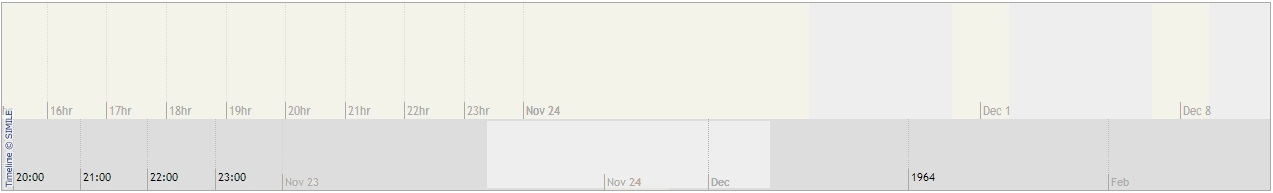
\includegraphics[width=150mm]{ge/tm1.jpg}
  \caption{Timeline}
  \label{fig:tm1}
\end{figure}

  \begin{figure}[H]
  \centering
    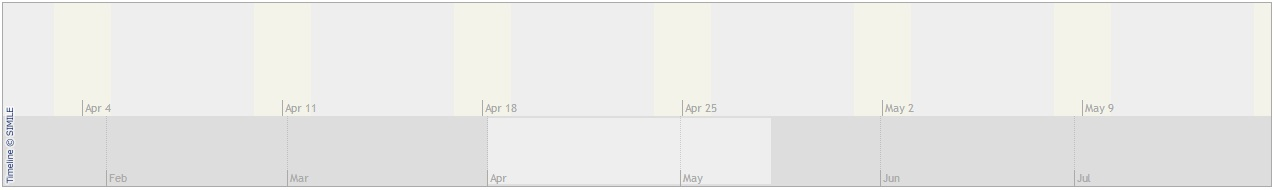
\includegraphics[width=150mm]{ge/tm2.jpg}
  \caption{Timeline 2}
  \label{fig:tm2}
\end{figure}

\subsubsection{Aktualizacja struktury DOM}
\label{subsubsec:dom}

Wszystkie elementy znajdujące się na stronie internetowej tworzą struktutę drzewa DOM(en.Document Object Model). Określa ono wzajemne położenie poszczególnych elementów, przy wykorzystaniu JavaScript-u możliwe jest akutalizowanie poszczególnych fragmentów strony bez konieczności renderowania wszystkich elementów.

Na rysunku \ref{fig:domtree} zaprezentowano minimalną struktturę wymaganą do poprawego korzystania z tworzonego projektu. W części head dodane są niezbędne odwołania do skttyptów które są odpowiedzialne za prawidłowe funkcjownowanie frameworku, do elementu body dołączono elementy ktore zapewniają miejsce dla wizualnej części, zdefiniowany rozmiar pozwala na precyzyjne wkompnowanie.

\begin{figure}[H]
  \centering
    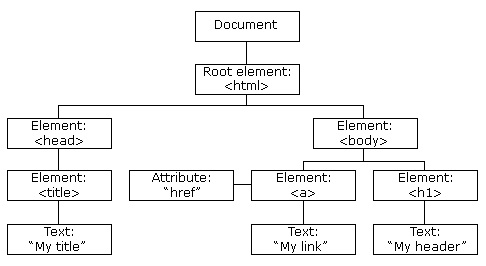
\includegraphics[width=100mm]{ge/htmltree2.jpg}
  \caption{Drzewo DOM}
  \label{fig:domtree}
\end{figure}
